\documentclass{patmorin}
\usepackage{amsthm,amsmath,graphicx,stmaryrd}
\usepackage{pat}

\DeclareMathOperator{\erf}{erf}
\newcommand{\eps}{\varepsilon}

\title{\MakeUppercase{On the Average Number of Edges in a Theta Graph}}
\author{Pat Morin,\thanks{School of Computer Science, Carleton University}\,\,
         and Sander Verdonschot\footnotemark[1]}



\begin{document}
\maketitle

\begin{abstract}
  The abstract goes here.
\end{abstract}

\section{Introduction}

Theta graphs, introduced by Keil \cite{A} and, independently by So and
So \cite{} are an important geometric structure that has applications
in networking \cite{A} and data structures.  For a point set, $S$, and
a positive integer, $k$, the $\theta_k$-graph, $\theta_k(S)$, of $S$
is an undirected geometric graph whose vertices are the points of $S$.
The edges of $\theta_k(S)$ are defined as ...

Theta graphs have two important properties that make them suited for
a wide variety of applications:  They are \emph{sparse}; $\theta_k(S)$
has at most $k|S|$ edges.  They are \emph{spanners}; the length of the
shortest path between any two vertices $u$ and $w$ is at most a constant
(dependant only on $k$ and not on $S$) times the Euclidean distance
between $u$ and $w$.  Keil \cite{kXX} showed that $\theta_k(S)$ is a
spanner for any $k\ge 7$, Bonichon \etal\ showed that $\theta_6(S)$
is a spanner,  Bose \etal\ showed that $\theta_5(S)$ is a spanner,
and Bose \etal\ \cite{bXX} showed that $\theta_4(S)$ is a spanner.
In contrast, it is easy to show that $\theta_k(S)$ is not necessarily
a spanner for $k\in\{1,2,3\}$.

Note that, although the $\theta_k(S)$ graph has at most $k|S|$ edges,
it can also have significantly fewer edges.  For example, if the points
of $S$ all lie on a line, then $\theta_k(S)$ has only $|S|-1$ edges.
More typical, though, is for a $\theta_k$-graph to have somewhere
between $k|S|/2$ and $k|S|$ edges;  each vertex $u\in S$ is responsible
for creating $k$ edges\footnote{Every vertex in $S$ creates $k$ edges
unless it is near the ``boundary'' of the point set.  More precisely,
only the points on the $(2\pi/k)$-hull \cite{alpha-hull} of $S$ may
create fewer than $k$ edges.} of the graph but sometimes an edge $uw$
is created both by $u$ and $w$.

In this paper, we study the typical number of edges in a $\theta_k$-graph
by studying the average number of edges in the $\theta_k$-graph of a
random point set.  A standard model for random point sets is a set of $n$
points independently and uniformly distributed in $[0,1]^2$.  In this
paper, however, we will consider points generated by a homogeneous Poisson
process with unit intensity over the entire Euclidean plane.  This is
done mainly to facilitate calculations; the extension of our results to
i.u.d.\ point sets in $[0,1]^2$ is discussed in \secref{summary}.

\subsection{The Model and Results}

In the Poisson model, the number of points in any region
whose area is $A$ follows a Poisson distribution with parameter $A$.
For definitions of Poisson processes and distributions see, for example,
Ross \cite[Chapter~2]{ross:introduction}.  For our purposes, the most
important properties of the Poisson process are the following:
\begin{enumerate}
\item The probability  that a particular region $X$ whose area is $A$
   is empty of points is exactly $e^{-A}$.
\item For two disjoint regions $X$ and $Y$, the events ``$X$ is empty
   of points'' and ``$Y$ is empty of points'' are independent.
\end{enumerate}
Note that, in this model, any $\theta$-graph will have an infinite number
of edges since there are an infinite number of points.  Therefore,
we study the average degree of a vertex in the $\theta$-graph.  For the
$\theta_k$-graph, this quantity is at most $2k$ since each vertex defines
$k$ edges of the graph and each edge has 2 endpoints.  However, in some
cases an edge $uw$ is \emph{mutual} in the sense that the edge is created
both by $u$ and by $w$.  If we let $p_k$ denote the probability that an
edge of the $\theta_k$ graph is is mutual, then the average degree of
the $\theta_k$ graph is
\[
    d_k = (2-p_k)k \enspace .
\]
Thus, understanding the average degree of a $\theta_k$-graph boils down
to computing $p_k$.

In \secref{even} we show that, for all even integers $k\ge 4$,
\[
    p_k=\frac{\pi\sqrt{3}}{9}\approx 0.6045997883 \enspace .
\]
That is, the probability of an edge being mutual is independent of
$k$. Thus, for all even integers $k\ge 4$, the average degree of a
vertex is
\[
  d_k = \left(2-\frac{\pi\sqrt{3}}{9}\right)k \approx 1.395400212\cdot k \enspace .
\]

In \secref{odd} we show that, for odd values of $k\ge 5$, the situation
is very different.  The mutual edge probability $p_k$ depends on
$k$ in a complicated way that includes trigonometric functions and
square roots.  However, the value of $p_k$ is significantly larger than
$\frac{\pi\sqrt{3}}{9}$ for all odd values of $k$.  Indeed, $p_k$ is a
decreasing function of $k$ and
\[
  p_k\ge \lim_{k\to\infty} p_k = 2\arctan(1/3)\approx 0.6435011088 \enspace .
\]
Thus, for all odd values of $k\ge 5$,
\[
   d_k \le (2-2\arctan(1/3))k \approx 1.356498891 k
\]
Thus, in some sense, odd values of $k$ offer ''more bang for the buck.''

In \secref{unit-square} we extend these results to points independently and uniformly distributed in a unit square.

\subsection{Related Work}

Devroye \etal. study the maximum degree of theta graphs and show that,
if $S$ is a set of $n$ points independently and uniformly distributed in
a certain unit square, then $\theta_k(S)$ has maximum degree concentrated
around $\Theta((\log n)/\log\log n)$.  In the Poisson model, their result
can be interpreted by fixing a $\sqrt{n}\times\sqrt{n}$ and counting
the maximum degree of any vertex in this square.



\section{An Analysis of $p_k$ for even $k$}
\seclabel{even}

In this section we determine the value of $p_k$ for even values of $k$.
Surprisingly, the value of $p_k$ in this case does not depend on $k$.

\begin{lem}\lemlabel{even}
 For even integers $k\ge 4$, $p_k=\frac{\pi\sqrt{3}}{9}\approx 0.6045997883$.
\end{lem}

\begin{proof}
  Let $u$ be an arbitrary vertex in a $\theta_k$ graph and let $w$
  be a vertex that $u$ has chosen as a neighbour in one of its cones,
  $C$ ($w$ is the ``closest'' vertex to $u$ in $C$).  Let $T$ be the
  open isosceles triangle defined by $C$ and a line
  through $w$ that is orthogonal to the axis of $C$. See \figref{mutual}.
  Observe that the location of $w$ is uniformly distributed on the
  edge of $T$ opposite $u$;  if this edge has length $\ell$, then $w$
  partitions it into two pieces of length $r$ and $\ell-r$, where $r$
  is uniformly distributed in $[0,\ell]$.

  \begin{figure}
    \centering{\includegraphics{cone}}
    \caption{The edge $uw$ is mutual if and only if $T'\setminus T$ 
       is empty of points.}
    \figlabel{mutual}
  \end{figure}
 
  Let $T'$ be the triangle obtained by reflecting $T$ through the midpoint
  of the edge $uw$ (so that $w$ is a vertex of $T'$). By Property~2 of the
  Poisson process, the edge $uw$ is mutual if and only if $T'\setminus T$
  contains no points.  The area of $T'\setminus T$ is
  \[
     A(T'\setminus T) = c(r^2+(\ell-r)^2)  \enspace ,
  \]
  where $c=c(k)$ depends only on $k$.  We now have enough information
  to compute the probability that the edge $uw$ is mutual conditional
  on $\ell$ and $r$:
  \[
    \Pr\{\mbox{$uw$ is mutual} \mid l,r\} = \exp(-c(r^2+(\ell-r)^2))
      \enspace .
  \]
  Since $r$ (conditioned on $\ell$) is uniform over $[0,\ell]$, unconditioning
  $r$ gives
  \begin{align*}
    f(\ell) & \equiv \Pr\{\mbox{$uw$ is mutual} \mid l\} \\
     & = \int_0^\ell (1/\ell)\exp(-c(r^2+(\ell-r)^2))\,\mathrm{d}r \\
     & = \frac{\sqrt{\pi}}{\ell\sqrt{2c}}
            \cdot\exp(-c\ell^2/2)
            \cdot\erf(\ell\sqrt{c/2})  \enspace ,
%     & = \sqrt{\frac{2\pi}{\sqrt{3}}}\exp(-\sqrt{3}\ell^2/8)
%         \cdot\erf(\sqrt[4]{3}\sqrt{2}\ell/4) \enspace ,
  \end{align*}
  where 
  \[ \erf(x)=\frac{2}{\sqrt{\pi}}\int_0^x e^{-t^2}\,\mathrm{d}t \]
  is the \emph{Gauss error function} \cite{gauss-error}.  

  Next, we remove the conditioning on $\ell$.  The triangle $T$ defines a
  region of area $c\ell^2$ that is empty of points.  Therefore,
  by Property~1 of the Poisson process, the cumulative distribution
  function of $\ell$ is given by
  \[
    P(x) \equiv \Pr\{\ell \le x\} = 1-\exp(-cx^2) \enspace .
  \]
  The probability density function of $\ell$ is therefore given by 
  \[
     p(x) \equiv \frac{d}{dx}P(x) =
     2cx\cdot\exp(-cx^2) \enspace .
  \]
  Finally, we obtain $p_k$ as 
  \begin{align*}
     p_k = \int_0^\infty p(\ell)\cdot f(\ell)\,\mathrm{d}\ell 
     = \frac{\pi\sqrt{3}}{9}
      \approx 0.6045997883  \enspace . & \qedhere
  \end{align*}
\end{proof}

Thus, for even $k$, the average degree of the $\theta_k$-graph is 
\[ d_k = \left(2-\frac{\pi\sqrt{3}}{9}\right)k \approx 1.395400212\cdot k \enspace . \]

\section{An Analysis of $p_k$ for $k$}
\seclabel{odd}

Next, we determine the value of $p_k$ for odd values of
$k\ge 5$.  Although the strategy for doing this is the same as the even
case, the odd case turns out to be considerably more complicated, and
we rely heavily on Maple for our calculations.

For the odd case the value of $p_k$ does, indeed depend on $k$.

\begin{lem}\lemlabel{odd}
  For odd $k\ge 5$,
\[
p_k = 
2
\left(\begin{array}{l}
  \arctan\left(
     2\left(\cos\left(\frac{\pi }{k}\right)
       +\cos\left(\frac{3 \pi }{k}\right)\right)^2 / (\alpha\beta) 
  \right) \\
   + \arctan\left(
       4 \left(2 \cos\left(\frac{2 \pi }{k}\right)
       +\sin\left(\frac{2 \pi }{k}\right)^2\right)/(\alpha\beta) 
     \right)
  \end{array}
\right)
%\\
\cot\left(\frac{\pi }{k}\right) 
\beta
%\right)
/
\left(\gamma \alpha\right)\enspace ,
\]
where
\[
\gamma =4+11 \cos\left(\frac{2 \pi }{k}\right)+\cos\left(\frac{6 \pi }{k}\right) \enspace ,
\]
\[
\alpha = 
\sqrt{\frac{\left(27 \cos\left(\frac{\pi }{k}\right)+17 \cos\left(\frac{3 \pi }{k}\right)+3 \cos\left(\frac{5 \pi }{k}\right)+\cos\left(\frac{7 \pi }{k}\right)\right) \csc\left(\frac{\pi }{k}\right)}{\gamma}} \enspace ,
\]
and
\[
\beta = \sqrt{\left(18 \sin\left(\frac{2 \pi }{k}\right)+18 \sin\left(\frac{4 \pi }{k}\right)+11 \sin\left(\frac{6 \pi }{k}\right)+\sin\left(\frac{8 \pi }{k}\right)+\sin\left(\frac{10 \pi }{k}\right)\right)} \enspace .
\]
\end{lem}

\begin{proof}
  The proof proceeds in the same manner as the proof of \lemref{even}.
  Let $u$ be an arbitrary vertex in a $\theta_k$ graph and let $w$ be
  a vertex that $u$ has chosen as a neighbour in one of its cones, $C$.
  Let $T$ be the open isosceles triangle defined by $C$ and a line through
  $w$ that is orthogonal to the axis of $C$. See \figref{mutual-odd}.
  Assume that the side of $T$ opposite $u$ has length $2\ell$.  Using a
  suitable rotation, we may assume that the axis of $C$ is horizontal and,
  by symmetry, we may assume that $w$ is on or above the axis of $C$.
 
  \begin{figure}
    \includegraphics{calcs}
    \caption{The derivation of the $\Pr\{\mbox{$uw$ is mutual}\mid \ell,r\}$
             for odd $k$.}
    \figlabel{mutual-odd}
  \end{figure}
  Under the preceding assumptions, $w$ is then uniformly distributed on
  a vertical segment of length $\ell$ whose endpoints are on the axis
  of $C$ and the upper boundary of $C$.  Suppose that the distance from
  $w$ to the axis of $C$ is $r$.  Then a straightforward, but tedious,
  calculation that mainly uses the law of sines shows that
  \[
      \Pr\{\mbox{$uw$ is mutual}\mid \ell, r\} = \exp(-A-B) \enspace ,
  \]
  where
  \[ 
      A = r^2\left(\frac{\cos(\pi/k)}{2\sin(\pi/k)}+\frac{\sin(\pi/k)}{\cos(\pi/k)}\right)
  \]
  and
  \[
      B = \frac{\left(\frac{\ell\cos(\pi/k)\sin(2\pi/k)}{\sin(3\pi/k)\sin(\pi/k)}-\frac{r\cos(2\pi/k)}{\sin(3\pi/k)}\right)^2\cos(2\pi/k)}{2\cos(\pi/k)}
  \]
  This calculation is illustrated in \figref{mutual-odd} and the
  accompanying Maple worksheet shows the simplifications that lead to
  the expressions for $A$ and $B$.  Integrating over $r$ gives us
  \begin{equation}
    \Pr\{\mbox{$uw$ is mutual}\mid \ell\} = 
      \int_0^\ell (1/\ell)\exp(-A-B)\,\mathrm{d}r . \eqlabel{odd-f}
  \end{equation}
  Like the corresponding integral in the proof of \lemref{even},
  \eqref{odd-f} has a closed-form that includes the Gauss error function.

  In order to remove the conditioning on $\ell$, we need the probability
  density function for $\ell$.  Proceeding as before, we have the
  cumulative distribution function
  \[
     P(x) \equiv \Pr\{\ell\le x\} 
          = 1 - \exp(\ell^2(\sin((\pi-\theta)/2)/\sin(\theta/2))) \enspace ,
  \]
  and the probability density function
  \[
    p(x)\equiv \frac{d}{dx}P(x) = 
     \left(\frac{2x\cos(\pi/k)}{\sin(\pi/k)}\right)
      \exp(x^2\cos(\pi/k)/\sin(\pi/k))
  \]
  Finally, we determine $p_k$ by integrating over $\ell$:
  \[
     p_k = \int_0^\infty p(\ell)\cdot f(\ell)\, \mathrm{d}{\ell} \enspace ,
  \]
  which (after introducing the variables $\alpha$, $\beta$, and $\gamma$)
  yields the expression for $p_k$ given in the statement of the lemma.
\end{proof}

\section{Points in a Unit Square}

Although we derive our results under the a Poisson model, in this section
we argue that similar results, albeit with lower-order error terms, hold
under the model of $n$ points independently and uniformly distributed
in the unit square $[0,1]^2$.

\begin{lem}
 Let $S$ be a set of $n$ points independently and uniformly distributed
 in $[0,1]^2$.  Then the expected number of edges in $\theta_k(S)$
 is $(2-p_k)kn/2\pm O(\sqrt{kn\log n})$.
\end{lem}

\begin{proof}[Proof Sketch]
The proof is essentially the same derivation used to prove
Lemmas~\ref{lem:odd} and \ref{lem:even} except that it uses a standard
trick (see, for example, Devroye \etal\ \cite{dgmXX}) of treating points
close to the boundary of the square differently from the remaining points.

To see this, observe that points sufficiently far from the boundary of
the unit square, say in $[c/\sqrt{n\log n},1-c/\sqrt{n\log n}]^2$ behave
essentially the same as points in the Poisson model.  In particular,
for any edge chosen by one of these points, the probablity that this edge
is mutual is $p_k\pm n^{-\Omega(c)}$.  

On the other hand, with high probability, the number of points near the
boundary of $[0,1]^2$ is only $\sqrt{n\log n}$.  The influence of these
points on the average degree of the $\theta_k(S)$ is therefore at most
$O((k\log n)/\sqrt{n})$.  Thus, the average degree of the $\theta_k$-graph
of points in the unit square is
\[  
 d_k' = (2-p_k)k\pm kn^{-\Omega(c)}+O((k\log n)/\sqrt{n}) \enspace .
\]
The expected number of edges is therefore:
\[
  nd_k'/2 = (2-p_k)kn/2\pm O((k\sqrt{n\log n}) \qedhere
\] 
\end{proof}

Next, we show that the number of edges in this model is tightly concentrated about its expected value:

\begin{lem}
 Let $S$ be a set of $n$ points independently and uniformly distributed
 in $[0,1]^2$ and let $m_k$ denote the number of edges in $\theta_k(S)$.
 Then $\Pr\{|m_k-(2-p_k)kn/2| \ge ck\sqrt{n\log n}\} \le e^{-\Omega(c)}$.
\end{lem}

\begin{proof}
First apply McDiarmid's inequality on the augmented $\theta_k$-graph
$\theta_k(S\cup Q)$, where $Q$ is a set of $k$ points at infinity.

Second, observe that, with high probability, the only differences between
$\theta_k(S)$ and $\theta_k(Q)$ is at boundary vertices, of which there
are only $O(\sqrt{n\log n}$.
\end{proof}





\section{Discussion}
\seclabel{summary}

We have given closed-form expressions for the average degree of $\theta_k$
graphs for all $k\ge 4$.  It is known that $\theta_k$-graphs with
$k=1,2,3$ do not have constant spanning ratios \cite{S}, so the cases
$k\ge 4$ are the most important.

\tabref{values} gives the numerical values of $d_k$, $p_k$, and $d_k/k$,
for $k\in\{4,\ldots,20\}$.  This table shows that odd values of $k$

\section*{Acknowledgement}

The authors of this paper are partly funded by NSERC and CFI.

\bibliographystyle{plain}
\bibliography{template}




\appendix

\section{Derivations for Even $k$}
\applabel{derivations-even}


\section{Derivations for Odd $k$}
\applabel{derivations-odd}
%\renewcommand{\left}[1]{#1}
%\renewcommand{\right}[1]{#1}



%\noindent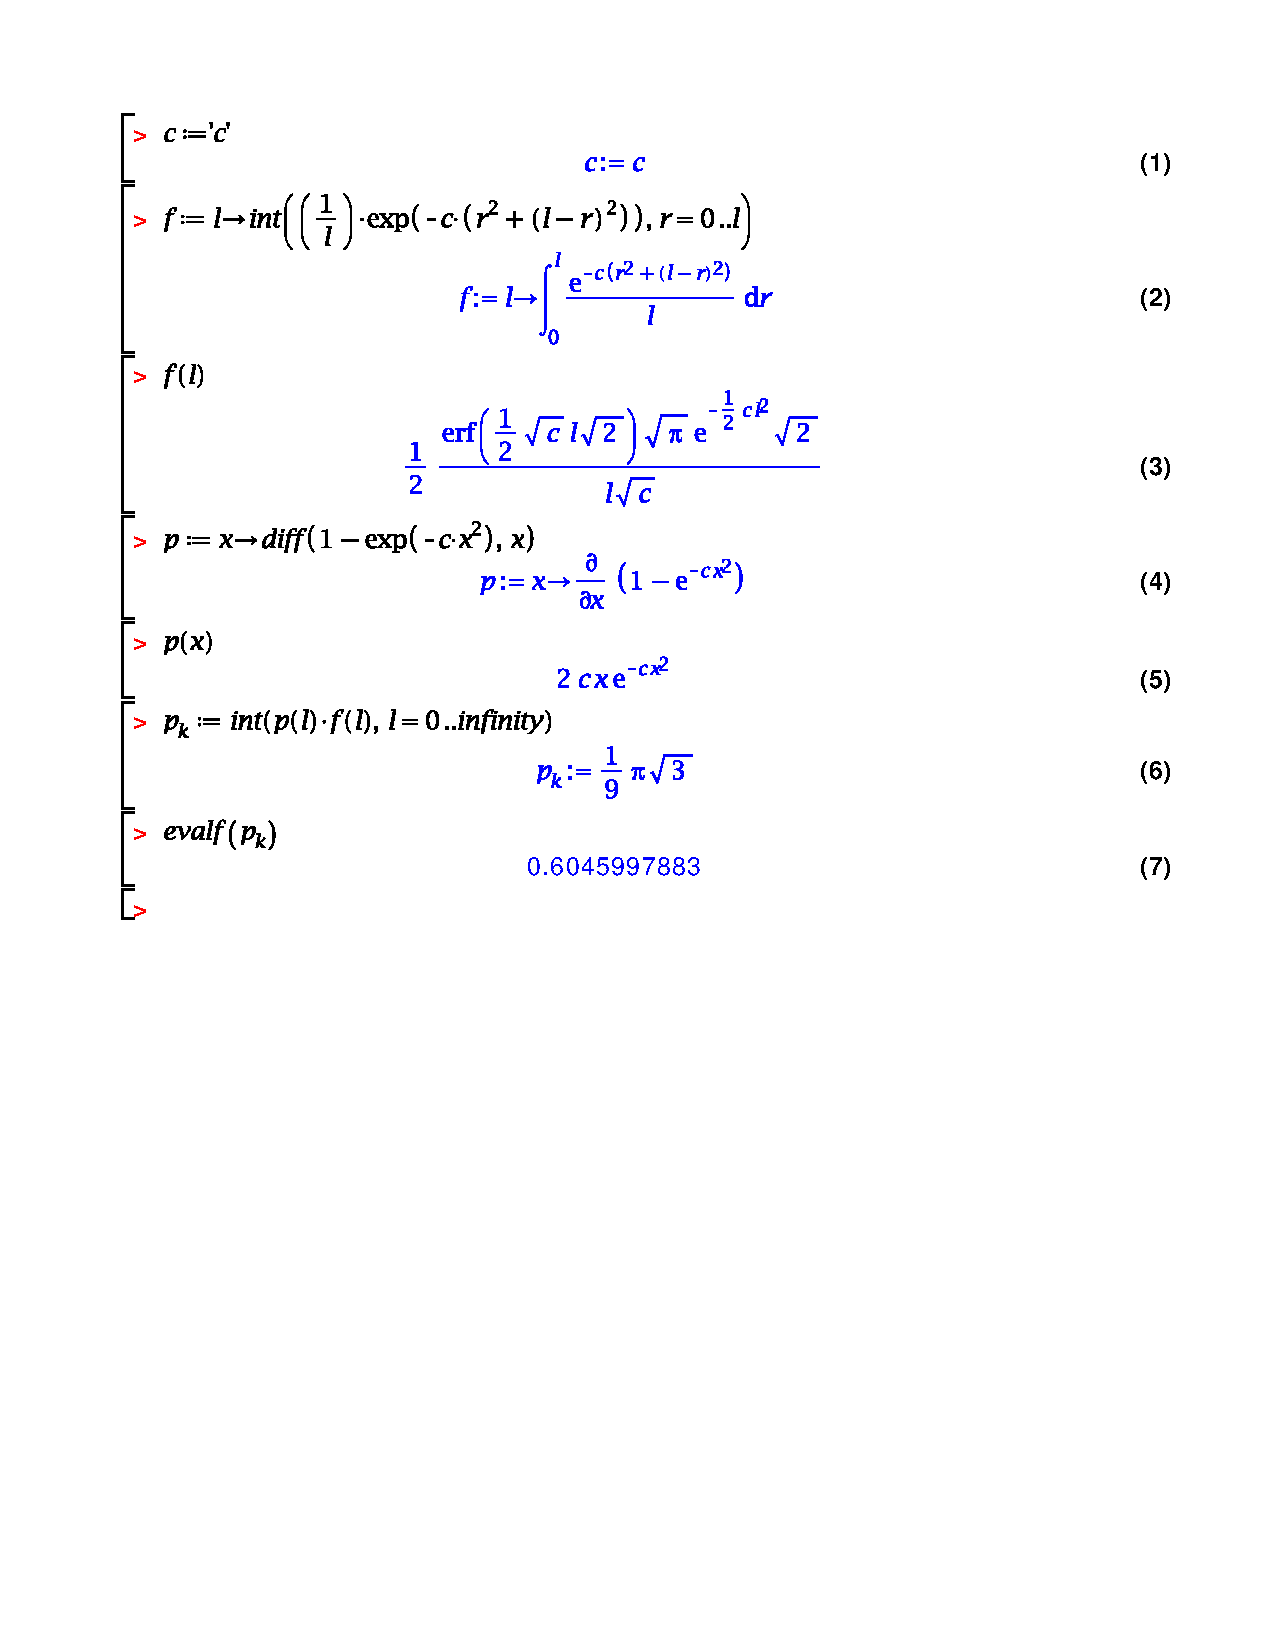
\includegraphics{even}


\end{document}


